%%
%% Author: Aga
%% 05.01.2019
%%

\documentclass{sprawozdanie-agh}

\usepackage[utf8]{inputenc}
\usepackage{listings}
\usepackage{pdfpages}
\usepackage{float}
\usepackage{anyfontsize}
\usepackage{graphicx}

\makeatletter 

\begin{document}   
	
	\przedmiot{Wprowadzenie do wzorców projektowych}
	\tytul{„Wzorce projektowe”}
	\podtytul{Implementacja server push w technice streaming}
	\kierunek{Informatyka, III rok, 2018/2019}
	\autor{Agnieszka Zadworny, Maciej Bielech, Tomasz Pęcak, Piotr Morawiecki}
	\data{Kraków, 13 grudnia 2018}
	
	\stronatytulowa{}
	
	\section{Informacje ogólne}

		\subsection{Cel projektu}
		Celem projektu jest zaimplementowanie metody Server Push w technice streaming przy użyciu technologii NodeJS i ReactJS.

		\subsection{Opis aplikacji}
		Utworzona została aplikacja webowa o nazwie ,,Tablica ogłoszeń'', która umożliwia publikowanie ogłoszeń o wybranej tematyce. Klient otwierając stronę aplikacji otrzymuje listę ogłoszeń sortowaną od najnowszego, jeśli w czasie przebywania na witrynie pojawi się nowe ogłoszenie, serwer wyśle jego treść dzięki wykorzystaniu techniki Server Push, która została zaimplementowana przy użyciu websocketów. 

		\subsection{Server Push}
		Push technology, czyli server push, to styl komunikacji internetowej, w którym żądanie danej transakcji jest inicjowane przez serwer. W przeciwieństwie do pull/get, gdzie żądanie przekazania informacji jest inicjowane przez odbiorcę lub klienta.

		Usługi Push są często oparte na preferencjach informacyjnych wyrażanych z wyprzedzeniem. Nazywa się to modelem publikacji/subskrybcji. Klient "subskrybuje" różne "kanały" informacyjne dostarczane przez serwer; gdy na jednym z tych kanałów dostępne są nowe treści, serwer "pushuje" te informacje do klienta.

		\subsection{Websocket}
		Protokół WebSocket umożliwia interakcję między klientem internetowym (np. przeglądarką), a serwerem WWW przy dokonywaniu mniejszej ilości zapytań, ułatwiając przesyłanie danych w czasie rzeczywistym z i na serwer. Jest to możliwe dzięki zapewnieniu znormalizowanego sposobu, w jaki serwer może wysyłać treści do klienta bez uprzedniego żądania z jego strony i pozwalającego na przekazywanie wiadomości w obu kierunkach przy zachowaniu otwartego połączenia. W ten sposób może mieć miejsce dwukierunkowe połączenie pomiędzy klientem i serwerem. 

		\begin{figure}[H]
			\centering
			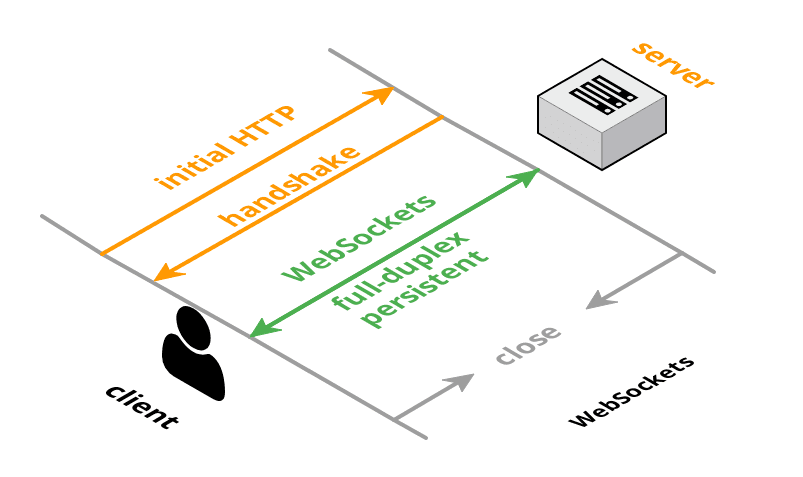
\includegraphics[scale=0.5]{websockets.png}
		\end{figure}
		
	\section{Diagramy}

	\begin{figure}[H]
		\centering
		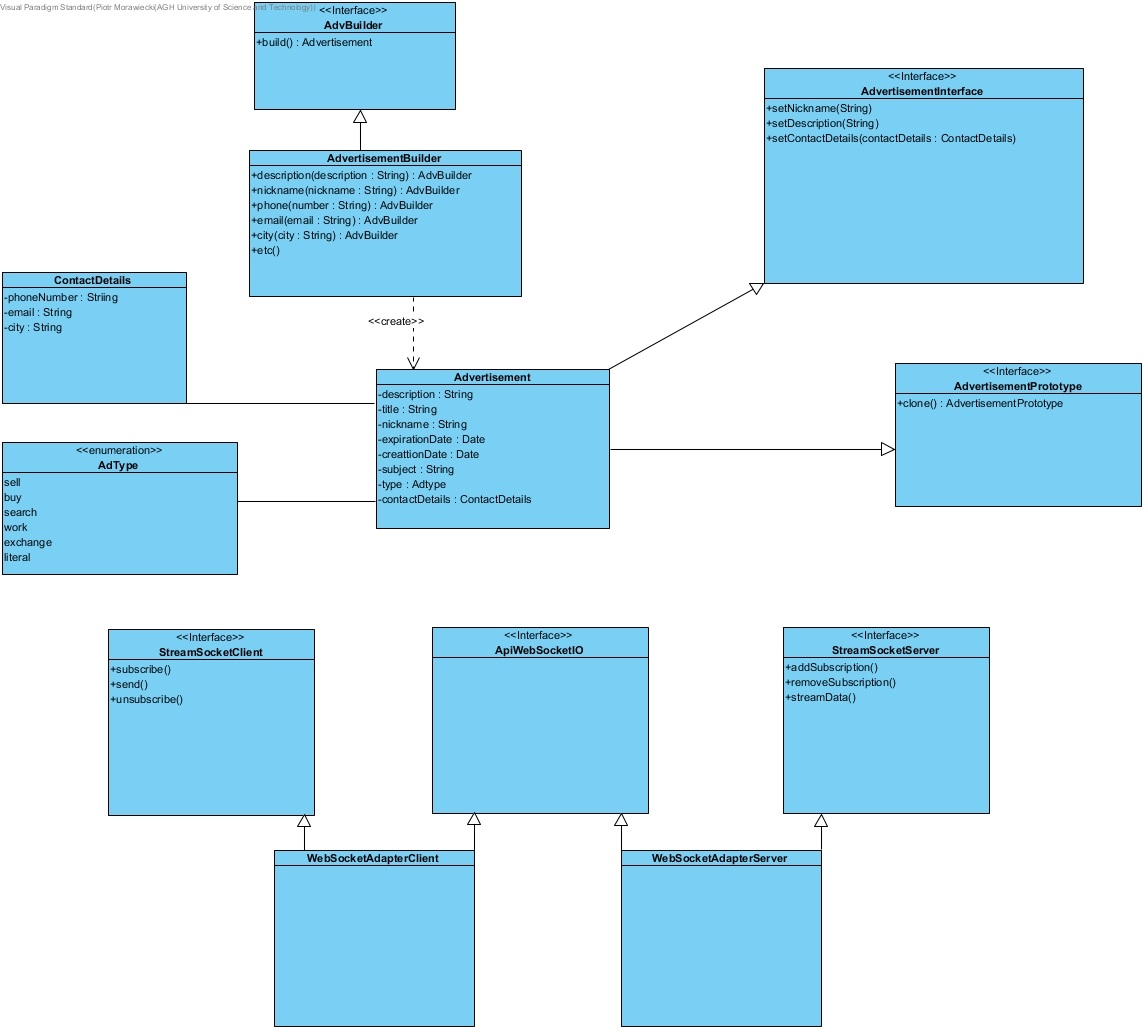
\includegraphics[scale=0.5]{prototype.jpg}
	\end{figure}
	\begin{figure}[H]
		\centering
		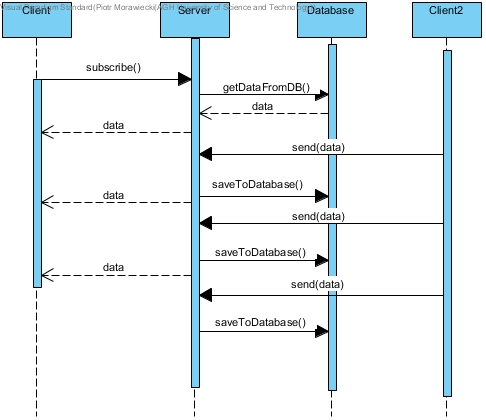
\includegraphics[scale=0.5]{sekwencyjny.jpg}
	\end{figure}
	\section{Wykorzystane wzorce projektowe}
		\subsection{Prototyp}
			Wykorzystanie wzorca \textit{prototyp} umożliwiło nam tworzenie nowych obiektów ogłoszenia zgodnie z ustalonym schematem z użyciem domyślnych wartości atrybutów klasy. Ogłoszenia charakteryzuje duża ilość domyślnych danych takich jak: czas utworzenia, typ, kategoria, anonimowa nazwa autora. Domyślna wartość czasu wygaśnięcia komunikatu została wprowadzona, aby ogłoszenia były aktualne. 
			\subsection{Builder}
			Ze względu na sporą ilość atrybutów opcjonalnych zdecydowaliśmy się skorzystać z wzorca \textit{builder}. Autorzy mogą decydować, które informacje chcą zamieścić na stronie. Dzięki temu proces tworzenia jest elastyczny i uwzględnia różne rodzaje ogłoszeń. 
			\subsection{Adapter}
			Z uwagi na wykorzystanie zewnętrznych bibliotek
			\textit{Socket.io} oraz \textit{Socket-Stream}, zdecydowaliśmy się skorzystać z wzorca \textit{adapter}, aby uzyskać jeden prosty interfejs łączący ich funkcjonalności. Umożliwiło to dostosowanie ich możliwości do naszych potrzeb, a tym samym znacząco uprościło to sposób korzystania z nich.
		
\end{document}